\documentclass[reprint,english,notitlepage]{revtex4-1}  % defines the basic parameters of the document

% if you want a single-column, remove reprint

% allows special characters (including æøå)
\usepackage[utf8]{inputenc}
\usepackage[english]{babel}


\newcommand*{\QEDA}{\hfill\ensuremath{\blacksquare}}
\usepackage{amsmath, amssymb}

%% note that you may need to download some of these packages manually, it depends on your setup.
%% I recommend downloading TeXMaker, because it includes a large library of the most common packages.

\usepackage{physics,amssymb}  % mathematical symbols (physics imports amsmath)
\usepackage{graphicx}         % include graphics such as plots
\usepackage{xcolor}           % set colors
\usepackage{hyperref}    
\usepackage{filecontents}
% automagic cross-referencing (this is GODLIKE)
\usepackage{tikz}             % draw figures manually
\usepackage{listings}         % display code
\usepackage{subfigure}        % imports a lot of cool and useful figure commands



% defines the color of hyperref objects
% Blending two colors:  blue!80!black  =  80% blue and 20% black
\hypersetup{ % this is just my personal choice, feel free to change things
    colorlinks,
    linkcolor={red!50!black},
    citecolor={blue!50!black},
    urlcolor={blue!80!black}}

%% Defines the style of the programming listing
%% This is actually my personal template, go ahead and change stuff if you want
\lstset{ %
	inputpath=,
	backgroundcolor=\color{white!88!black},
	basicstyle={\ttfamily\scriptsize},
	commentstyle=\color{magenta},
	language=Python,
	morekeywords={True,False},
	tabsize=4,
	stringstyle=\color{green!55!black},
	frame=single,
	keywordstyle=\color{blue},
	showstringspaces=false,
	columns=fullflexible,
	keepspaces=true}

%% USEFUL LINKS:
%%
%%   UiO LaTeX guides:        https://www.mn.uio.no/ifi/tjenester/it/hjelp/latex/ 
%%   mathematics:             https://en.wikibooks.org/wiki/LaTeX/Mathematics

%%   PHYSICS !                https://mirror.hmc.edu/ctan/macros/latex/contrib/physics/physics.pdf

%%   the basics of Tikz:       https://en.wikibooks.org/wiki/LaTeX/PGF/TikZ
%%   all the colors!:          https://en.wikibooks.org/wiki/LaTeX/Colors
%%   how to draw tables:       https://en.wikibooks.org/wiki/LaTeX/Tables
%%   code listing styles:      https://en.wikibooks.org/wiki/LaTeX/Source_Code_Listings
%%   \includegraphics          https://en.wikibooks.org/wiki/LaTeX/Importing_Graphics
%%   learn more about figures  https://en.wikibooks.org/wiki/LaTeX/Floats,_Figures_and_Captions
%%   automagic bibliography:   https://en.wikibooks.org/wiki/LaTeX/Bibliography_Management  (this one is kinda difficult the first time)
%%   REVTeX Guide:             http://www.physics.csbsju.edu/370/papers/Journal_Style_Manuals/auguide4-1.pdf
%%
%%   (this document is of class "revtex4-1", the REVTeX Guide explains how the class works)


%% CREATING THE .pdf FILE USING LINUX IN THE TERMINAL
%% 
%% [terminal]$ pdflatex template.tex
%%
%% Run the command twice, always.
%% If you want to use \footnote, you need to run these commands (IN THIS SPECIFIC ORDER)
%% 
%% [terminal]$ pdflatex template.tex
%% [terminal]$ bibtex template
%% [terminal]$ pdflatex template.tex
%% [terminal]$ pdflatex template.tex
%%
%% Don't ask me why, I don't know.
\begin{document}
\title{FYS-STK4155 H22: Project 1 \\ \vspace{}
\large{Modelling 3D terrain using Linear Regression.}}
\author{Lasse Totland, Domantas Sakalys, Synne Mo Sandnes}
\date{\today}      % self-explanatory
\noaffiliation                            % ignore this
\begin{abstract} %abs?
This report compares various methods for regression analysis and resampling techniques by applying them to three-dimensional data-sets; one set is randomly generated as $z = f(x,y) + \epsilon$ where $f(x,y)$ is the Franke function and $\epsilon$ is added normal-distributed noise with variance $\sigma^2 = 0.1$, the other dataset is actual terrain data. From our Ridge and Lasso analysis of the Franke function we found that the optimal regularization parameter tends to be $\lambda = 0$, leading us to conclude that an OLS approximation is sufficient. From a bias-variance analysis we determined that an appropriate polynomial degree for this model would be a value in the range of $N \in [4, 10]$ to avoid under- and overfitting. From our analysis of the terrain data we reached the same conclusions. Additionally, we found that Ridge starts to make significant adjustments when we introduce higher amounts of noise to the data and can be more viable than OLS in such cases.
\end{abstract}                            % marks the end of the abstract
\maketitle                                % creates the title, author, date & abstract


% the fundamental components of scientific reports:

\section{Introduction} 

This report demonstrates and compares various methods for regression analysis and resampling techniques by applying them to three-dimensional data-sets; one set semi-randomly generated and the other a real set of terrain data. We will use different methods, like evaluating mean square error, score ($R^2$) and bias-variance trade-off analysis to quality check the resulting regression models and decide on the optimal one for our case. Learning to reach correct conclusions from the results of these methods can be a great tool in data analysis to develop numerical models that are efficient, and avoid subtle but unfortunate side-effects like under- and overfitting.

\section{Theory}

Some of the formulae presented in this report have been borrowed from the task descriptions' original LaTeX file. \hfill \footnote{FYS-STK4155 Project 1 H22, Morten Hjorth-Jensen}

Borrowed figures are marked as such with citations, and figures made by us are not.

\subsection{Franke Function}

The Franke function, which is a weighted sum of four exponentials reads as
follows:

\begin{figure}[h!]
    \centering
    \includegraphics[scale = 0.215]{franke.PNG}
\end{figure}

For a two-dimensional xy-plane input, the function gives us a 'terrain' plot.

\subsection{Mean Square Error (MSE)}

% Kommentar: You do not give any insights or interpretation to what the MSE is


The Mean Square Error (MSE) of an approximated model $\tilde{\bm{y}}$, given the inital data ${y}$ can be expressed:

\[ MSE(\bm{y}, \ \tilde{\bm{y}}) = \frac{1}{n}
\sum_{i=0}^{n-1}(y_i-\tilde{y}_i)^2, 
\] 

where $n$ is the number of values in $\tilde{\bm{y}}$.\\

\subsection{Score Function, $R^2$}

The score function can be used to determine the quality of our model. If $\tilde{\bm{y}}_i$ is the predicted value of the $i'th$ sample and $y_i$ is the corresponding true value, then the score $R^2$ is defined as

\[
R^2(\bm{y}, \tilde{\bm{y}}) = 1 - \frac{\sum_{i=0}^{n - 1} (y_i - \tilde{y}_i)^2}{\sum_{i=0}^{n - 1} (y_i - \bar{y})^2},
\]

where we have defined the mean value  of $\bm{y}$ as

\[
\bar{y} =  \frac{1}{n} \sum_{i=0}^{n - 1} y_i.
\]

The score function can have values in the range $R^2 \in [0, 1]$ where $R^2 = 1$ would mean that $\tilde{y}$ was a perfect fit of $y$.

\subsection{Ordinary Least Squares (OLS) method}

Given a dataset with $n$ values in the form $y = f(x) + \epsilon$, where $\epsilon \sim N(0, \ \sigma^2)$ is normally distributed noise, $f(x)$ can be approximated via the development of a model of the form:

\begin{equation} \label{eq:predict}
    \tilde{y} = \bm{X}\beta
\end{equation}


$X \in \mathbb{R}^{n \times p}$ is a design matrix with columns representing the different features $p$ of the model. For a simple second degree polynomial, the resulting model may look like this:

$$\tilde{y} = \beta_0 + x\beta_1 + x^2\beta_2.$$

$\beta$ is thus a column vector with an amount of scalar values $\beta_i \ (i \in [0, p])$ representing specific features. The OLS method defines it as:



\begin{align}
    \label{ols}
    \beta^{OLS} = (X^TX)^{-1}X^Ty.
\end{align}


\subsection{Ridge method}



\footnote{\label{ref1} Morten Hjorth-Jensen. Applied Data Analysis and Machine Learning. Copyright 2021. \url{https://compphysics.github.io/MachineLearning/doc/LectureNotes/_build/html/intro.html}} The matrix $X^TX$ may sometimes be singular, making it incapable of being inverted. The OLS method will not work in this case, as the matrix in equation \ref{ols} is inverted. This can be a result of independent variables having a high degree of correlation. Ridge regression can be used to make the matrix non-singular. A parameter $\lambda$ is then added to the diagonal.







For Ridge regression, the cost function is


\begin{align}
    C(\boldsymbol{\beta})=\sum_{i=0}^{p-1}(y_i-\beta_i)^2+\lambda\sum_{i=0}^{p-1}\beta_i^2,
\end{align}


Ridge regression reduces the values of of $\beta_i$  as a function of $\lambda$. \\ The Ridge penalty squares the individual model parameters. This indicates that the larger values are weighted significantly more heavily than the smaller ones. Thus, ridge regression prioritizes minimizing large model parameters over small model parametres. This is an advantage as long as the values we are working with are small, because then they don’t need to be reduced any further. 



Ridge regression uses a modified definition of $\beta^{OLS}$:


\begin{equation}\label{eq:ridge}
    \beta^{Ridge} = (X^TX + I\lambda)^{-1}X^Ty
\end{equation}


Here $I^{p \times p}$ is the identity matrix, and $\lambda \geq 0$ is a regularization parameter that is basically used to fine tune the OLS regression model. If $\lambda = 0$, that means that the OLS model is a good model for the approximation; no fine-tuning required. \\





\subsection{Lasso method}

\footnotemark[\value{footnote}] Another adaption of the linear regression is the Lasso regression ('Least Absolute Shrinkage and Selection Operator'). This method is used to get a more accurate prediction by changing the cost function. The result is a model more robust against overfitting. \\

The cost function for the Lasso method is defined

\begin{align}
    C(\boldsymbol{\beta})=\sum_{i=0}^{p-1}(y_i-\beta_i)^2+\lambda\sum_{i=0}^{p-1}\vert\beta_i\vert \\ =\sum_{i=0}^{p-1}(y_i-\beta_i)^2+\lambda\sum_{i=0}^{p-1}\sqrt{\beta_i^2}
\end{align}





Lasso regression uses a modified definition of $\beta$:

$$\beta^{Lasso}_i = \begin{cases}
    (y_i - \frac{\lambda}{2}), & \text{if  } y_i > \frac{\lambda}{2}\\
    (y_i + \frac{\lambda}{2}), & \text{if  } y_i < -\frac{\lambda}{2}\\ 
    0, & \text{if  } \abs{y_i} \leq \frac{\lambda}{2}.
\end{cases},$$

where $\lambda$ is a regularization parameter as in the Ridge method. \\


Lasso regression sets values of $\beta_i$ to zero for specific values of $\lambda$. This is useful as it makes it possible to discard unimportant predictors. \\




The Lasso penalty takes the absolute model parameters. This leads to the large and small values being taken equally into account. In contrast to the ridge regression, it does not prioritize minimizing any particular model parameter. 

\subsection{The Cost function}

% Kommentar: You do not give any insights or interpretation to what the cost function is

Given a model $\tilde{\bm{y}}$, approximating data $\bm{y} = f(x) + \epsilon$, its corresponding parameters $\bm{\beta}$ are in turn found by optimizing the mean squared error via the so-called cost function, which we have rewritten as:

\[
C(X,\beta) = \mathbb{E}\left[(\bm{y}-\bm{\tilde{y}})^2\right]=(\mathrm{Bias}[\tilde{y}])^2+\mathrm{var}[\tilde{y}]+\sigma^2, 
\]

where $var[\tilde{y}]$ and $\sigma^2$ are the variances of the model and the noise respectively, representing the spread of these data. The square of the bias of the model represents error from wrong assumptions in the model; one can think of a model with high bias to have an inherent systematic error. Figure \ref{fig:bv1} presents a useful visualization of how variance and bias of a model relate. The derivation of the equation above is presented in Appendix A.

The terms represent different potential sources of error in our model, so the cost function can be used to detect this and minimize the mean square error.

\begin{figure}[h!]
    \centering
    \includegraphics[scale = 0.33]{biasvar.PNG}
    \caption{Visualization of the dynamic between bias and variance in a model. The intent of this model would be to hit the red bullseye in all instances. \footnote{'Understanding the Bias-Variance trade-off', Scott Fortmann-Roe (2012) \url{http://scott.fortmann-roe.com/docs/BiasVariance.html}}}
    \label{fig:bv1}
\end{figure}

\subsection{Bias-variance trade-off}

The details of the relation between the bias and variance of a model is interesting as well, and can tell us something about the optimal complexity of the model. Complexity in regression analysis refers to the polynomial degree of the model attempt. The 'trade-off' refers to a compromise; we mostly cannot reduce both the error from the bias and the variance to its minimum, but we can determine a middle-point that sufficiently avoids \textit{overfitting} and \textit{underfitting}.

\begin{figure}[h!]
    \centering
    \includegraphics[scale = 0.5]{biasvariance.png}
    \caption{Visualization of the dynamic between bias, variance and total error in a model as a function of model complexity. \footnote{'Understanding the Bias-Variance trade-off', Scott Fortmann-Roe (2012)}}
    \label{fig:bv2}
\end{figure}

In Figure \ref{fig:bv2} we can see how the optimal model complexity is determined to be at the minimum total error (about where the bias and variance cross). Decreasing the complexity from here leads to underfitting; the model does not have the sufficient parameters to accomplish a good fit. Increasing the complexity from the 'sweet spot' also increases error as the model gains more features but also most likely gains more spread in the model data.

A bias variance plot most likely won't be as smooth as this example figure and the optimal complexity won't be as obvious, so we may have to compare with other methods to make a good evaluation.

\subsection{Resampling methods}

While analyzing a limited dataset it may be useful to 'resample' it; create subsets of the original data with new variations (for example by replacing values) and then analyze those as well and evaluate how this extends the model. The intent of resampling is essentially to have more data to work with during analysis. We're going to use two such methods for this project.

The \textit{bootstrap method} involves generating additional datasets $y_i$ from an original $y$, where a larger range of $i$'s would mean a more thorough evaluation. The additional sets resample randomly chosen values from the original, and analyzing all of these sets will give a distribution of predicted models where the mean is determined to be the optimal one. In regression analysis for example, we'll get a distribution of $\beta_k$'s that represent approximation models.

When developing approximation models it may be useful to divide the data $y$ into a \textit{training} set to build the model, and keep a spare \textit{test} set to evaluate the quality of the model; a sufficient model should be able apply itself to new data. The \textit{Cross-validation method} mixes up how this is structured, and generates a sequence of $k$ equally sized groups from a shuffled subset $y_i$ of $y$, and determines one of these to be the test set. Analyzing all of these training/test-set groups will give a distribution of models, where the mean is determined be the optimal one.



\section{Method}

We generate the data that will be analyzed by inserting uniformly generated points $x, y \in [0, 1]$, inserting into Franke function $f(x, y)$ and then adding stochastic, normal-distributed noise $\epsilon \sim N(0, \ \sigma^2)$. We define the dataset as:

$$z = f(x, y) + \epsilon,$$

assuming a variance of $\sigma^2 = 0.1$. See Figure \ref{fig:noise} for an example of how the generated data may look.

\begin{figure}[h!]
    \centering
    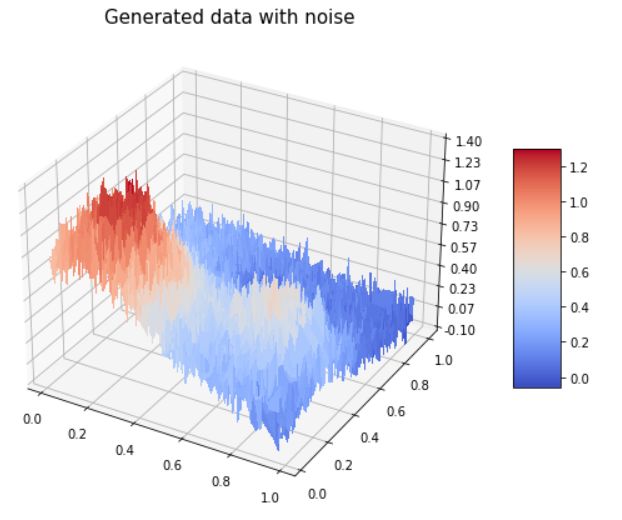
\includegraphics[scale = 0.33]{project1b_noisydata.PNG}
    \caption{An example of generated data $\textbf{z}$ from Franke function as described in the method section. This specific terrain was generated with a resolution of a $100 \times 100$ xy-grid.}
    \label{fig:noise}
\end{figure}

\subsection{Applying the Ordinary Least Squares (OLS) analysis}
We wish to approximate the initial function $f(x, y)$ with our model $\tilde{z}$ following from the OLS-method:

$$\tilde{z} = X\beta,$$

where $X$ is the design matrix determined by the polynomial degree of our model. The form of our design matrix will correspond to a multiple polynomial regression model, meaning each feature of our $\beta$ will be a product of various degrees of $x^i, y^i$ for $i \in [1, N]$ where $N$ is the polynomial degree of our regression. For $N = 1$ for example, our model will have three features and may look like this (including intercept):

$$\tilde{z} = \beta_0 + x\beta_1 + y\beta_2 + xy\beta_3.$$

The python function for constructing the design matrices ('create\_X') is borrowed from the lecture notes \footnote{Applied Data Analysis and Machine Learning lecture notes H22 subsection 4.8, Morten Hjorth-Jensen}, and can be found in the attached jupyter notebook with our code.

With a defined design matrix, we can can find $\beta^{OLS}$ as defined in the theory section, giving us a complete model $\tilde{z} = X\beta$.

We'll use several strategies to evaluate the quality of our model. Firstly we'll split the data into 'training' and 'test' sets. More specifically, we are going to assign 80\% of the data $z$ and the same percentage of the rows in $X$ to the training set, and use it to develop our model (calculate $\beta$), then use the remaining 20\% to see if the finished model is in correspondence with the remaining data.

To quantitatively evaluate this we'll calculate the Mean Square Error ($MSE$) and the Score Function ($R^2$) for the training and test data sets and compare. We'll use the definitions presented in the theory section.

We'll also take into account the polynomial degree N of our OLS regression. A higher degree N will give the model more features, and more parameters to adjust the model to the data, but we'll have to evaluate if the added model complexity gives meaningful improvement or if it leads to overfitting (the model tries to fit to the noise and not the data 'underneath').

To do this we'll compare $MSE$ and $R^2$ as functions of model complexity $N$. In addition, we will compare $var[\beta]$ as function of $N$, which represents the spread of elements in the $\beta$ column-vector, and may also show signs of overfitting.

\subsection{Bias-Variance trade-off analysis}

To help us further determine to optimal model complexity (polynomial degree N) we'll also perform a bias-variance trade-off analysis, as described in the theory section. As a function of N, we'll plot the error, bias and variance and attempt to determine from this plot what degree N minimizes over- and underfitting.

The script used for this analysis will be an extended version of a script presented in the lecture notes (subsection 5.4) which demonstrates bias-variance analysis of a two dimensional function (and implements a bootstrap method), which we will expand to function for three dimensional OLS models.

We will also compare the error from the mentioned resampling techniques (Bootstrap and Cross-validation) and see if we can use what we know to determine which method is most optimal for our analysis. The implementation of cross-validation is also derived from a script in the lecture notes (5.5), extended to resample for every polynomial degree in OLS in three dimensions.

\subsection{Ridge method implementation}

For the Ridge method implementation, we wish to tweak the parameter $\lambda$ in equation \ref{eq:ridge}, and find which value gives least mean square error. We choose an array of values ranging from -15 to 15 on a logarithmic scale. The number of elements in this array is 100. We then make a loop, where we take each value of lambda and calculate the $\beta^{\text{Ridge}}$ as done in equation \ref{eq:ridge}. By having $\beta^{\text{Ridge}}$, we proceed in the same loop to calculate the predicted z-array by equation \ref{eq:predict}, but now by using $\beta^{\text{Ridge}}$.\\
\\
Additionally, we scale our data. We do this after we split the dataset into training and testing set. We use 80\% of data as training set, and the rest 20\% as training set. We take this training set, and subtract the mean value of this this training set.
$$X_{\text{train, scaled}} = X_{train} - <X_{train}>$$
$$z_{\text{train, scaled}} = z_{train} - <z_{train}>$$
We use these scaled sets to determine $\beta^{\text{Ridge}}$.
However, when calculating the predicted values, we use the testing $X_{train}$ set from which we subtract the mean value of training set $<X_{train}>$. Additionally, we add a term to the predicted values. The predicted value expression is
$$z_{pred} = (X_{test} - <X_{train}>) + z_{\text{train, scaled}}$$
We then proceed to calculate the mean square error for the this predicted set $z_{pred}$ with their own values of $\lambda$. 









\subsection{Lasso method implementation}
As for the Lasso implementation, we follow the same steps as we did with Ridge implementation. Here however, we use sklearn python library \footnote{https://scikit-learn.org/stable/modules/linear_model.html} in order to find the predicted values for $z$. We once again, scale the data here as well. 

\subsection{Terrain data analysis}

After our analysis work on the Franke function, we'll apply what we've learned on real terrain data. We've chosen to work with one of the given datasets 'SRTM\_data\_Norway\_1.tif'. The dataset contains $3601 \times 1801$ altitude-values from an area close to Stavanger, Norway. This is a lot larger than the Franke dataset we worked with and would take a lot of time to analyze, so we'll focus on a smaller area to make the script run more efficiently.

We decided on a smaller section of resolution $100 \times 100$ to perform the regression analysis on, this terrain can be seen in Figure \ref{fig:terrain}. We've also normalized the altitudes between $[0, 1]$ so the errors will be in a comparable scale with our previous work on the Franke function.

The reason for such a small resolution is due to the lengthy script. In it we're already implementing three different regression techniques, 25 lambda values in a range of $\lambda \in log[-15, 15]$, and 5 kfolds in the cross-validation analysis. For a large selection of data, the runtime of all of this increases many-fold, which we don't have the time to wait for.

\begin{figure}[h!]
    \centering
    \includegraphics[scale = 0.48]{terrain.png}
    \caption{$100 \times 100$ meter resolution Terrain plot from Stavanger, altitude (originally in meters above sea level) normalized.}
    \label{fig:terrain}
\end{figure}

With this data we are going to compare the performance of the different regression methods we've established (OLS, Ridge, Lasso) by calculating the error as function of model complexity as done previously.

The script 'Terrain\_data\_g.ipynb' contains all of the analysis work on the terrain data.

To conclude, we'll discuss the applicability of these regression methods. There may not be one method that is superior to the others in all cases (how does performance vary with the size of the datasets?), but we'll see if we can identify their respective strengths and weaknesses through our results and see if one method is more ideal for our case of three dimentional terrain analysis. 

\section{Results}

\subsection{Results from Ordinary Least Squares analysis}

To understand the comparisons of model quality as function of complexity, it may be useful to see what the resulting OLS regression models look like for different polynomial degrees. In Figure \ref{fig:ols_approx} (Appendix B) we demonstrate how increasing the degree from 2 to 5 gives a gradually more complex terrain, and that the higher degrees seem like more accurate recreations of the initial noisy terrain.

Figure \ref{fig:5} and \ref{fig:6} present the $MSE$ and $R^2$ from a run of the script, respectively, as functions of model complexity. Figure \ref{fig:varb} shows the variance of $\beta$ as function of model complexity from the same run, as a way to compare the beta-parameters. Additionally, see Figure \ref{fig:fig5_modded} in appendix section for comparison of MSE calculated by a model with and without bootstrap resampling method.

\begin{figure}[h!]
    \centering
    \includegraphics[scale = 0.54]{MSE.png}
    \caption{Mean Square Error of the OLS regression on the Franke function training and test sets as function of polynomial degree N.}
    \label{fig:5}
\end{figure}

\begin{figure}[h!]
    \centering
    \includegraphics[scale = 0.54]{R2.png}
    \caption{Score Function $R^2$ of the OLS regression on the Franke function training and test sets as function of polynomial degree N.}
    \label{fig:6}
\end{figure}

\begin{figure}[h!]
    \centering
    \includegraphics[scale = 0.54]{varb.png}
    \caption{The variance $var[\beta]$ of the OLS regression on the Franke function training and test sets as function of polynomial degree N.}
    \label{fig:varb}
\end{figure}

\subsection{Bias-Variance trade-off analysis of OLS}

Figure \ref{fig:bias} shows a result from bias-variance analysis of OLS approximations of Franke function as functions of model complexity N. For this run, the xy-grid had a resolution of $40\times 40$ points, and the variance of the noise determined as $\sigma^2 = 0.1$. The script producing this plot also implemented 100 bootstrap iterations to resample the initial data for every polynomial degree.

\begin{figure}[h!]
    \centering
    \includegraphics[scale = 0.55]{B-V.png}
    \caption{Error, bias and variance of OLS approximations of Franke function as functions of model complexity N.}
    \label{fig:bias}
\end{figure}

\subsection{Comparison of resampling techniques}

Figure  \ref{fig:crossboot} shows a comparison of the mean square error of a run of OLS regressions of the Franke function at increasing polynomial degrees (model complexity). The script implements 10 k-folds in the cross validation resampling, the data and the bootstrap set-up was defined exactly how it was in the bias-variance analysis. It may seem like the cross-validation method is more successful here (it generally has lower MSE), but this varied greatly between different runs of the script. This is just one example.

\begin{figure}[h!]
    \centering
    \includegraphics[scale = 0.55]{bootcross.png}
    \caption{Mean Square Error of OLS regression using Bootstrap and Cross Validation compared as function of model complexity N.}
    \label{fig:crossboot}
\end{figure}


\subsection{Ridge method analysis}
By plotting mean square error with different values of $\lambda$'s, we get the following plot in figure \ref{fig:ridge}

\begin{figure}[h!]
    \centering
    \includegraphics[scale = 0.85]{ridge.png}
    \caption{Plot for Ridge analysis for lambdas in range from $10^{-15}$ to $10^{15}$}
    \label{fig:ridge}
\end{figure}

In Figure \ref{fig:ridge}, it is clear that the MSE drops for low non zero values of lambda. This indicates that the extra term of $I\lambda$ in equation \ref{fig:5} for $Beta^{ridge}$ must be zero, in order to have the best approximation to the noisy Franke's function. When $\lambda$ is zero, the Ridge Beta becomes the same Beta as it is for OLS. 
$$\beta^{ridge} = \beta^{OLS}$$
This result shows that the OLS is a good approximation for the data, and there is no need to tweak the $\beta$ parameter with $\lambda$

\subsection{Lasso method analysis}
By plotting mean square error with different values of $\lambda$'s and by using Lasso approximation, we get the following plot as shown in Figure \ref{fig:lasso}.

\begin{figure}[h!]
    \centering
    \includegraphics[scale = 0.85]{lasso.png}
    \caption{Plot for Lasso analysis for most optimal $\lambda$ value. Same as in Ridge analysis, we get $\lambda = 0$ to be the most optimal.}
    \label{fig:lasso}
\end{figure}

\subsection{Results from terrain data analysis}

Figure \ref{fig:terrain_analysis} shows the resulting mean square error from regressions at increasing model complexity N, with different regression techniques. Cross-validation resampling with 5 kfolds was also applied. The OLS and Ridge methods mostly overlap, until N = 10. The Lasso regression 'lags' behind and performs worse from N = 3 and onwards.

\begin{figure}[h!]
    \centering
    \includegraphics[scale = 0.55]{CrossRegr.png}
    \caption{Comparison of error of approximations of terrain data using different regression methods, with applied cross-validation resampling, as functions of model complexity N.}
    \label{fig:terrain_analysis}
\end{figure}

We also calculated the $MSE$ and $R^2$ scores for each of the methods respective training and test data, which can be seen in Figure \ref{fig:terrain_misc} in Appendix B. Those plots yield a similar result as seen in Figure \ref{fig:terrain_analysis}.

\section{Discussion}

When discussing the results of regression analysis of the Franke function in this report, its important to keep in mind that the datasets used were randomly generated (as described previously) giving slightly varying data, models and results during quality check. Each run of our script generates a new dataset and the figures presented in this report are the results of one such run, not a decisive and final representation of its qualities.

Despite the random effects on our analysis, there are patterns and distinctive tendencies with the results of each of the different methods however, which is what we will discuss.

\subsection{Ordinary Least Squares analysis}

Studying Figure \ref{fig:5} and \ref{fig:6}, it is apparent that the mean square error $MSE$ of the models decrease, and that the score function $R^2$ increases, as the models become more complex (higher polynomial degrees N). This begs the question; if we keep increasing N, will our model improve after every step?

In Figure \ref{fig:OLS_ext} in Appendix B we have extended the $MSE$ and $R^2$ plots up to N = 13, and the first thing we notice is that the change after N = 5 is fairly small, but the score function undoubtedly increases a little bit for each step.

However, comparing the test and training $R^2$ score, we should also notice how the training data departs from the test data, and the test data consistently scores worse than the training after N = 4. This can be a sign of overfitting, i.e. the model tries too hard to fit to our noisy data $z = f(x,y) + \epsilon$ instead of the underlying function $f(x, y)$ that we are trying to approximate.

Lets revisit our OLS bias-variance trade-off analysis (see Figure \ref{fig:bias}), that was also performed on the same generated data as Figure \ref{fig:OLS_ext} (same parameters, same 'random seed' in script, giving the same random values every run). We see that the error and bias overlap up until N = 5, and depart from eachother afterwards. We clearly don't have an obvious N that corresponds to a perfect balance between under- and overfitting (as visualized in Figure \ref{fig:bv2} in the theory section with a distinct minimum) as the drastic signs of overfitting don't occur before around N = 11 where the error starts to skyrocket.

We can, however, conclude from this analysis that polynomial degrees in the range of around $N \in [4, 10]$ are respectable choices for a OLS model of the Franke function in regards to avoiding under- and overfitting.

The choice of a specific N in this range comes down to performance. Larger model complexity means larger matrices that must be handled, and a longer script running time. In our case, the amount of data we have from the Franke function is small enough that our choice is not very consequential.

Regarding our comparisons of the boostrap and cross-validation resampling methods (Figure \ref{fig:crossboot}) none of them seem to give decisively superior results, as mentioned already. It is worth pointing out that our 100 bootstrap iterations took longer to compute than the 10 kfold iterations. So with efficiency in mind, we can consider the cross-validation method as more favourable.

\subsection{Ridge method analysis}
From figure \ref{fig:ridge} we can clearly see that there is no need for any tweaking in OLS-method. OLS-method is very good to approximate our data. However, by increasing the noise of our vanilla data, we find that the optimal $\lambda$ is no longer 0. As this Figure \ref{fig:ridge_noise} shows.

\begin{figure}[h!]
    \centering
    \includegraphics[scale = 0.85]{ridge_noise.png}
    \caption{Ridge $\lambda$ analysis with higher noise}
    \label{fig:ridge_noise}
\end{figure}

In this figure, we can see that the optimal $\lambda$ is approximately 5.8. However, we have increased the noise significantly. Figure \ref{fig:high_noise} shows the plot of Franke's function with this new noise.
\begin{figure}[h!]
    \centering
    \includegraphics[scale = 0.5]{high_noise.png}
    \caption{Franke's function with high noise of $\sigma^2 = 1$ }
    \label{fig:high_noise}
\end{figure}
It is rare that we get such data with this much noise. It is more reasonable to get data set that has less noise, and looks more like Figure \ref{fig:noise}. This is why it is not necessary to increase the noise of our vanilla data in order to study ridge more in depth.



\subsection{Lasso method analysis}
We see that Lasso analysis for $\lambda$ agrees with the analysis with Ridge. We therefore can say that OLS approximation method is a good model for our data. Once again if we increase the noise in our vanilla data, we no longer get $\lambda = 0$ for Lasso. However, as discussed earlier, this is not necessary. 

\subsection{Application on terrain data}

In Figure \ref{fig:terrain_analysis} the OLS and Ridge regression models of the terrain data seem to give the smallest amount of error, except at N = 10 and onwards where the Ridge method seems to start adjusting noticeably.

This is good proof that the OLS method is a good choice of model for this data, considering that the Ridge model doesn't surpass the OLS score until N = 10 as it probably doesn't gain much from it. The adjustments may be that the Ridge model attempts to counter the overfitting (that we've seen occur around this range of polynomial degrees for the OLS model earlier). For even higher degrees we observe the OLS curve 'bounce' over and under the Ridge curve until it settles beneath it with a smaller error. At this point though, as we've previously concluded, the models are prone to overfitting so the higher range doesn't really interest us much and OLS should be a perfectly sufficient and effective model at lower degrees from what we've seen.

The Lasso model performs consistently worse than the other two from N = 4 and onwards with a higher error, though the difference is honestly quite small. It is reasonable to conclude that any of the methods are decent choices but why this clear and sudden difference after overlapping with OLS and Ridge up until N = 4? 

It may be because the Lasso method prefers models with fewer features, and we didn't do any extra modifications to our data to account for this. We may also have used the lasso function wrong, \textit{or} this is actually a reasonable result and Lasso just performs best at low degrees and never surpasses OLS with such smooth data.

\section{Conclusion}

In this report we have compared various methods for regression analysis and resampling techniques by applying them to three-dimensional data-sets; one set randomly generated and the other actual terrain data. From our Ridge and Lasso analysis of the Franke function generated data we found that the optimal regularization parameter tends to be $\lambda = 0$, leading us to conclude that an OLS approximation is sufficient. From a bias-variance analysis we determined that an appropriate polynomial degree for this model would be a value in the range of $N \in [4, 10]$ to avoid under- and overfitting. From our analysis of the terrain data we reach the same conclusions. Additionally, we found that Ridge starts to make significant adjustments when we introduce higher amounts of noise to the data and is more viable than OLS in such cases.

The fact that we reached the same conclusion with several different methods of regression and quality check, on two fairly similar datasets, is a good indicator that our conclusions are reasonable. If we theoretically had more time to work on this project, it could be interesting to have a more detailed look into scenarios where Ridge and Lasso regression were more viable than OLS, and study how they compare to eachother then.

\section{Appendix A: Derivations}


    \subsection{Variance of $\beta$}

    We have made the assumption that there exists a continuous function $f(\mathbf{x})$ and a normal distributed error $\boldsymbol{\varepsilon}$ $\sim N(0, \sigma^2)$ which describes our data

    $$\mathbf{y} = f(\mathbf{x}) + \boldsymbol{\varepsilon} = \mathbf{\tilde{y}} + \boldsymbol{\varepsilon}= X \mathbf{\beta} + \boldsymbol{\varepsilon}$$

    where the function $f(\mathbf{x})$ is approximated with the model $\mathbf{\tilde{y}}$ from the solution of the linear regression equations. The X is the design matrix. \\


    We will be showing that the expectation value of $\mathbf{y}$ for a given element i is 


    $$\mathbb{E}(y_i) = \sum_j x_{ij} \beta_j = \mathbf{X}_{i,*} \mathbf{\beta}$$

    We have that

    $$\mathbb{E}(y_i) = <y_i> = <\sum_j x_{ij} \beta_j + \boldsymbol{\varepsilon_i}>$$

    Because of linearity, we have $<\sum_j x_{ij} \beta_j> + <\boldsymbol{\varepsilon_i}>$

    The first term sums over the whole row on column i. This means that the content must be a scalar, and the expected value of a scalar is a scalar itself. \\

    As for the second term, $<\boldsymbol{\varepsilon_i}>$, we have assumed that $\boldsymbol{\varepsilon} \sim N(0, \sigma^2) \Rightarrow <\boldsymbol{\varepsilon}> = 0 \Rightarrow <y_i> = \sum_j x_{ij} \beta_j$



    We will now be showing that the variance of $\mathbf{y}$ is 
    $$Var(y_i) = \sigma^2$$
    
    The variance is a measurement of how much each number in our data differs from $mean(\mathbb{E}(y_i))$  

    $$<(y_i - <y_i>)^2>$$

    Because of linearity, we can write this
    
    \begin{gather*}    
     <y_i^2 - 2y_i <y_i>^2 > \\ = \;  <y_i^2> - <2y_i <y_i>> + <<y_i>^2> \\
    = \; <y_i^2> - <y_i><2y_i> + <y_i>^2 \\ 
    = \; <y_i^2 - 2<y_i><y_i> + <y_i^2> \\  =  \; <y_i^2> - 2<y_i>^2 + <y_i>^2 \\
    = \; <y_i^2> - <y_i>^2
    \end{gather*}

    We know that $$(y_i) =  \; <\sum_j x_{ij} \beta_j + \boldsymbol{\varepsilon_i}>$$

    \begin{gather*}
        \Rightarrow  \; <(\sum_j x_{ij} \beta_j + \boldsymbol{\varepsilon_i})^2> - (\sum_j x_{ij} \beta_j)^2 \\
        =  \; <(\sum_j x_{ij} \beta_j)^2 + 2  \sum_j x_{ij} \beta_j \boldsymbol{\varepsilon}_i + \boldsymbol{\varepsilon}_i^2)> - (\sum_j x_{ij} \beta_j)^2 \\
        =  \; <(\sum_j x_{ij} \beta_j)^2> + 2  \sum_j x_{ij} \beta_j <\boldsymbol{\varepsilon}_i> + <\boldsymbol{\varepsilon}_i^2> - (\sum_j x_{ij} \beta_j)^2 \\
        =  \; <\boldsymbol{\varepsilon}_i^2>  \; =   \sigma^2
    \end{gather*}


    This means that $y_i \sim N(\mathbf{X}_{i,*}\boldsymbol{\beta}, \sigma^2)$, telling us that $\mathbf{y}$ follows a normal distribution with mean value $\mathbf{X} \beta$ and variance $\sigma^2$. \\

    Will now show that $\mathbb{E}(\boldsymbol{\hat{\beta}}) = \boldsymbol{\beta}$. \\

    We can express $\boldsymbol{\beta} = (\mathbf{X}^T\mathbf{X})^{-1}\mathbf{X}^T \mathbf{y}$ \\ $$\Rightarrow  <(\mathbf{X}^T\mathbf{X})^{-1}\mathbf{X}^T \mathbf{y}>$$ \\

    \vspace{-5pt}
    
    Factor $(\mathbf{X}^T\mathbf{X})^{-1}\mathbf{X}^T$ is a matrix of constants, hence we can write \\

    
    
    $$<(\mathbf{X}^T\mathbf{X})^{-1}\mathbf{X}^T \mathbf{y}> = (\mathbf{X}^T\mathbf{X})^{-1}\mathbf{X}^T< \mathbf{y}>$$ \\

    

    again, we write $\mathbf{y} = \mathbf{X} \boldsymbol{\beta} + \boldsymbol{\varepsilon}$, and  \\ $$<\mathbf{X} \boldsymbol{\beta} + \boldsymbol{\varepsilon}> = \mathbf{X}< \boldsymbol{\beta}> + <\boldsymbol{\varepsilon}>$$ \\

    \vspace{-40pt}

    \[ \Rightarrow (\mathbf{X}^T\mathbf{X})^{-1}\mathbf{X}^T (\mathbf{X}< \boldsymbol{\beta}> + <\boldsymbol{\varepsilon}>) \] \\

    \vspace{-40pt}

    \[ = (\mathbf{X}^T\mathbf{X})^{-1}\mathbf{X}^T \mathbf{X}\boldsymbol{\beta} + (\mathbf{X}^T\mathbf{X})^{-1}\mathbf{X}^T <\boldsymbol{\varepsilon}> = \mathbb{I} \boldsymbol{\beta} = \boldsymbol{\beta} \] \\

    %where we have used the result 

    %this is wrong, as we are using that E(beta)=beta to show that E(B)=B

    
    This result means that the estimator of the regression is unbiased. \\


    We will now show that the variance of $\boldsymbol{\beta}$ is \\

    $$\mathrm{Var}(\boldsymbol{\hat{\beta}}) = \sigma^2 (\mathbf{X}^T \mathbf{X})^{-1}$$

    
    
    For this derivation, we use the following

    $$\mathrm{Var}(AB) = A \mathrm{Var}(B) A^T$$

    where B is a stochastic matrix, and A is not a stochastic matrix. Now \\

    $$\Rightarrow \mathrm{Var}(\boldsymbol{\hat{\beta}}) = \mathrm{Var}((\mathbf{X}^T\mathbf{X})^{-1}\mathbf{X}^T\mathbf{y})$$

    
    $(\mathbf{X}^T\mathbf{X})^{-1}\mathbf{X}^T$ is a non stochastic matrix, while $\mathbf{y}$ is stochastic. 

    $$\Rightarrow \mathrm{Var}(\boldsymbol{\hat{\beta}}) = (\mathbf{X}^T\mathbf{X})^{-1}\mathbf{X}^T \mathrm{Var}(\mathbf{y})[(\mathbf{X}^T\mathbf{X})^{-1}\mathbf{X}^T]^T$$

    We also use the following relations:

    $(AB)^T = B^TA^T$ and $(A^{-1})^T = (A^T)^{-1}$. \\

    Then 
    $$[(\mathbf{X}^T\mathbf{X})^{-1}\mathbf{X}^T]^T = (\mathbf{X}^T)^T((\mathbf{X}^T\mathbf{X})^{-1})^T = \mathbf{X}(\mathbf{X}^T\mathbf{X})^{-1}$$

    $$\Rightarrow \mathrm{Var}(\boldsymbol{\hat{\beta}}) = (\mathbf{X}^T\mathbf{X})^{-1}\mathbf{X}^T (\sigma^2 \boldsymbol{I}) \mathbf{X} (\mathbf{X}^T\mathbf{X})^{-1}$$


    $$= \sigma^2 (\mathbf{X}^T\mathbf{X})^{-1}\mathbf{X}^T  \mathbf{X} (\mathbf{X}^T\mathbf{X})^{-1} = \sigma^2(\mathbf{X}^T\mathbf{X})^{-1}$$\\

\subsection{The Cost function}

The given cost function was defined as

\[
C(\bm{X},\bm{\beta}) =\frac{1}{n}\sum_{i=0}^{n-1}(y_i-\tilde{y}_i)^2=\mathbb{E}\left[(\bm{y}-\bm{\tilde{y}})^2\right].
\]
Here the expected value $\mathbb{E}$ is the sample value. Given $y = f + \epsilon$ we can equate:

$$\mathbb{E}\left[(\bm{y}-\bm{\tilde{y}})^2\right] = \mathbb{E}\left[(f + \epsilon -\bm{\tilde{y}})^2\right]$$

$$\mathbb{E}\left[(\bm{y}-\bm{\tilde{y}})^2\right] = \mathbb{E}\left[(f + \epsilon -\bm{\tilde{y}} + \mathbb{E}[\tilde{y}] - \mathbb{E}[\tilde{y}])^2\right].$$

This multinomial expansion becomes long and tedious, but can be simplified if we keep in mind that all terms with a factor $\epsilon$ or $\mathbb{E}[\epsilon]$ become zero (the expectation value of normal distributed noise with mean value zero gives zero). The remaining terms are:

$$ = \mathbb{E}[(y - \mathbb{E}[\tilde{y}])^2] + \mathbb{E}[\epsilon^2] + \mathbb{E}[(\mathbb{E}[\tilde{y}] - \tilde{y})^2]$$

$$=(\mathrm{Bias}[\tilde{y}])^2+\mathrm{var}[\tilde{f}]+\sigma^2. \quad \quad \quad \quad \QEDA$$

Here we also used that $(Bias[\tilde{y}])^2 = (y - \mathbb{E}[\tilde{y}])^2$ and that $var[\tilde{f}] = \frac{1}{n}\sum_i(\tilde{y}_i-\mathbb{E}\left[\bm{\tilde{y}}\right])^2$.

\section{Appendix B: Additional figures}

\onecolumngrid
\begin{figure}[h!]
    \centering
    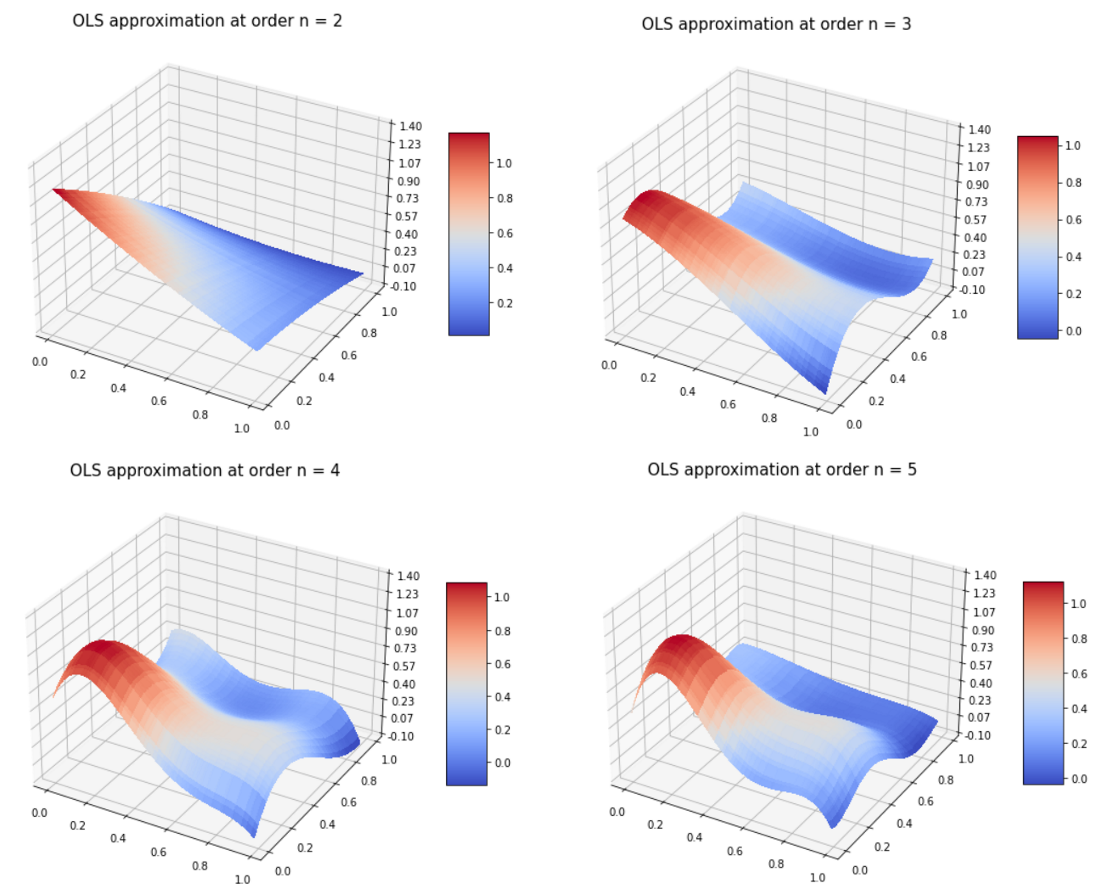
\includegraphics[scale = 0.5]{project1b_approx.PNG}
    \caption{OLS regression models using increasing polynomial degrees to approximate a generated Franke function terrain data set as the one seen in Figure \ref{fig:noise}.}
    \label{fig:ols_approx}
\end{figure}

\begin{figure}[h!]
    \centering
    \includegraphics[scale = 0.65]{MSE_R2_13.png}
    \caption{$MSE$ and $R^2$ from OLS regression (as seen in Figure \ref{fig:5} and \ref{fig:6}) for a larger range of polynomial degrees. These plots also correspond to a smaller dataset of $40 \times 40$ xy-grid (The same setup as we used for our bias-variance analysis of the OLS model). The MSE plot is reminiscent of Fig 2.11 of Hastie et al., as the test error ends up larger than the training error.}
    \label{fig:OLS_ext}
\end{figure}

\begin{figure}[h!]
    \centering
    \includegraphics[scale = 0.7]{c_start.png}
    \caption{Plot of MSE as a function of polynomial approximation degree. It is clear that approximation with bootstrap resampling method is almost no better than simple approximation without bootstrap. It has used 100 n-bootstrap loops. }
    \label{fig:fig5_modded}
\end{figure}
\twocolumngrid

\begin{figure}[h!]
    \centering
    \includegraphics[scale = 0.6]{MSE_R_ORL.png}
    \caption{$MSE$ and $R^2$ from a run of the script as functions of model complexity, comparing OLS, Ridge and Lasso regression. The Ridge values largely overlap the OLS values, their largest divergence (Ridge has about 0.002 higher $R^2$ score at $N = 12$ than OLS) can be seen if studied closely.}
    \label{fig:terrain_misc}
\end{figure}

\end{document}

